\title{Pendolo invertito su rotaia}
\maketitle
\label{sec:pic}


\section{Introduzione}
\paragraph{Il pendolo invertito su rotaia è un sistema facile da modellare,}
ma presenta alcune caratterische che rendono interessante studiarne la controllabilità.
Il sistema è mostrato in figura \ref{fig:pic} e consiste in un pendolo rigido, libero di ruotare e vincolato a muoversi lungo una rotaia rettilinea tramite un carrello. L'unico modo in cui i sistema può interagire con l'esterno è tramite una forza applicata sul carrello lungo la direzione della rotaia. Quando il pendolo è fermo ed è diretto verso l'alto, si trova in un punti di equilibrio instabile e ogni minima perturbazione tenderà a farlo ricadere verso il basso. L'obiettivo che mi pongo è duplice:

\begin{enumerate}
    \item Stabilizzare il pendolo attorno al punto di equilibrio instabile, in modo che sia resistente alle perturbazioni.
    \item Trovare una strategia per portare il pendolo in prossimità del punto di equilibrio instabile, partendo dalla configurazione stabile (\emph{swing-up}).
\end{enumerate}

%todo traduci in italiano
\paragraph{Il sistema è non-lineare e underactuated.} Questo significa che per portare a termine i due obiettivi discussi sopra, è necessario unire le due strategie di controllo discusse nei capitoli \ref{sec:linear-control}  e \ref{sec:nonlinear-control}. Inoltre, un singolo input deve essere in grado di controllare un sistema a due gradi di libertà: la posizione del carrello e l'angolo del pendolo, rientrando nei limiti di lunghezza della rotaia. In questo paragrafo creerò un modello del sistema e lo userò sia per dimostrare che è possibile effettuare lo swing-up del pendolo, sia per disegnare controller LQR per stabilizzarlo. Mostrerò quindi che è possibile raggiungere l'obiettivo che mi sono posto mettendo assieme le due strategie di controllo. Per concludere, userò il modello per stimare alcuni parametri del sistema reale.

%todo
\begin{figure}[thb]
    \centering
    %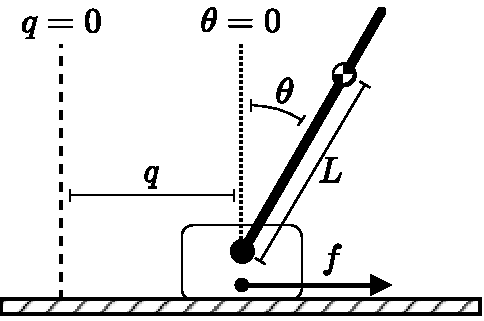
\includegraphics[width=0.4\textwidth]{assets/pic.png}
    \caption{Pic system. Qui ci va tutta la figura e la descrizione del sistema. }%todo
    \label{fig:pic}
\end{figure}




\section{Modello del sistema}
Nel paragrafo precedente ho detto che l'unica interazione possibile tra il sistema è l'esterno è l'applicazione di una forza sul carrello. Nella pratica, questo significa che è presente un motore vincolato al carrello in qualche modo. Mentre la natura del vincolo non è interessante, dobbiamo invece prestare particolare attenzione al tipo di motore utilizzato. Un motore esercita una forza che dipende sia da un segnale di controllo esterno, sia dallo stato interno dello stesso. È quindi conveniente separare lo studio del sistema in due: pendolo-carrello e motore.

\begin{figure}[thb]
    \centering
    %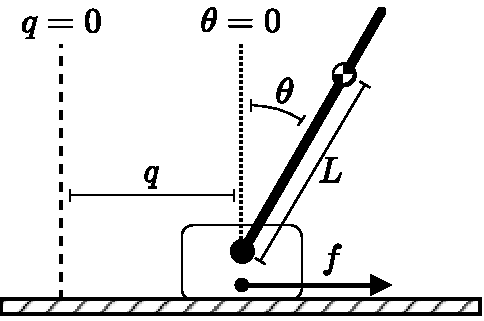
\includegraphics[width=0.4\textwidth]{assets/pic.png}
    \caption{Pic system. Qui ci va circa la stessa figura sopra, ma con l'immagine del motore collegato al carrello. }%todo
    \label{fig:pic-real}
\end{figure}

\subsection{Pendolo e carrello}
È immediato ricavare le equazioni del moto usando l'approccio Lagrangiano. Inizio fissando alcuni parametri che possono essere misurati sperimentalmente; sono riportati in tabella \ref{tab:parametri}. Posso quindi scrivere l'espressione per l'energia cinetica $T$ e potenziale $V$ del sistema:

\begin{equation*}
    \begin{aligned}
    T &= \frac 1 2 M  \dot q^2 +  \\ %todo
    V &= mgL \cos\theta
    \end{aligned}
    \hspace{20pt} \text{con } q \in \R, \theta \in ]-\pi, +\pi].
    \label{eq:energy}
\end{equation*}
La Lagrangiana $\mathcal L$ è data da:
\begin{equation*}
    \mathcal L = T - V
\end{equation*}
e posso ricavare le equazioni del moto usando le equazioni di Eulero:
\begin{equation*}
    \begin{aligned}
    asdasdasd %todo scrivi eq eulero
    \end{aligned}.
    \label{eq:moto-sistema}
\end{equation*}
%todo
Qui ci dovrei mettere due considerazioni sulle forze (in particolare sugli attriti...)
Studio inoltre i punti di equilibrio del sistema:
\begin{equation*}
    \left. \frac \partial {\partial \theta}\right |_{V=V_{eq}} V =  0 \implies V_{eq} = \{0, \pi\}.
\end{equation*}


\begin{table}[htbp]
    \centering
    \begin{tabular}{@{}ll@{}}
        \toprule
        \textbf{Correct}     & \textbf{Incorrect}         \\
        \midrule
        \( A \implies B \)   & \( A \Rightarrow B \)      \\
        \( A \impliedby B \) & \( A \Leftarrow B \)       \\
        \( A \iff B \)       & \( A \Leftrightarrow B \)  \\
        \bottomrule
    \end{tabular}
    % Tra graffe ci sta il nome che viene visualizzato nell'elenco delle tabelle
    \caption[Parametri]{Parametri}
    %todo
    \label{tab:parametri}
\end{table}
\todo{fai tabella}

\subsection{Motore}
\todo{fix reference}
\ref{https://homepages.laas.fr/lzaccari/seminars/DCmotors.pdf}
Per questa applicazione è sufficiente usare un motore DC a spazzole. Il motore è attivato applicando una differenza di potenziale $U$ tra le due armature e il verso di rotazione dipende dal segno della differenza di potenziale. Variando $U$ si ottiene grossolanamente un controllo sulla velocità di rotazione. Io voglio controllare la forza che il motore esercita sul carrello e devo quindi trovare la relazione tra differenza di potenziale e coppia $\tau$.
Fisso alcuni parametri relativi al motore, riportati in tabella \ref{tab:parametri-motore}.

\begin{table}[htbp]
    \centering
    \begin{tabular}{@{}ll@{}}
        \toprule
        \textbf{Correct}     & \textbf{Incorrect}         \\
        \midrule
        \( A \implies B \)   & \( A \Rightarrow B \)      \\
        \( A \impliedby B \) & \( A \Leftarrow B \)       \\
        \( A \iff B \)       & \( A \Leftrightarrow B \)  \\
        \bottomrule
    \end{tabular}
    % Tra graffe ci sta il nome che viene visualizzato nell'elenco delle tabelle
    \caption[Parametri motore]{Parametri motore}
    %todo
    \label{tab:parametri-motore}
\end{table}
\todo{fai tabella}


Un motore DC è regolato dalle equazioni: \todo{qui devo ritrovare il pdf che spiega tutto bene e decidere se fare io i disegni o se citare semplicemente altri paper}
\begin{equation*}
    \left\{ 
        \begin{aligned}
            U &= L_a \dot J + R_a J + K_e \omega \\
            \tau &= K_m J
        \end{aligned}
    \right.
    .
\end{equation*}

La coppia è proporzionale alla corrente che scorre nel motore. Si possono realizzare diversi circuiti di alimentazione che controllano direttamente la corrente ma il sistema che ho realizzato nella sezione \ref{sec:sistema-reale} può solo controllare il voltaggio. In più, il sistema non ha un sensore per misurare la corrente che passa nel motore.
Per trovare una soluzione al mio problema inizio risolvendo il sistema per $U$:
\begin{equation*}
    \begin{aligned}
    U &= L_a \partiald t \left(\frac \tau {K_m}\right) + R_a \frac \tau {K_m} + K_e \omega \\
      &= \frac {L_a} {K_m} \dot\tau + \frac{R_a}{K_m}  \tau + K_e \omega.
    \end{aligned}
\end{equation*}
In linea di principio questo è tutto quello che mi serve per controllare il motore, tuttavia, il termine che contiene $\dot \tau$ ha un coefficiente che non è facile da misurare con gli strumenti che ho a disposizione. Scelgo quindi di trascurare questo termine. Questa scelta è giustificata dal fatto che il segnale di controllo $\tau$ cambia solamente ogni $\Delta t$ secondi e posso scegliere $\Delta t$ in modo che sia maggiore del tempo del transiente dovuto a $\Delta \tau$.

Ricordando che $\tau$ e $\omega$ sono proporzionali a $f$ e $v$, trovo che questo modello dipende solo da due parametri determinabili sperimentalmente, $A$ e $B$:
\begin{equation*}
    U = A f + B v.
\end{equation*}
La determinazione di questi parametri è descritta nel paragrafo \ref{subsec:parametri-motore}.



\section{Realizzazione del sistema nel mondo reale}
\label{sec:sistema-reale}
Qui ci metto schemi, foto, considerazioni su come ho costruito le robe. Ci metto anche una tabella dei parametri e alcune considerazioni su come mai ho scelto proprio certi parametri. Tipo, le considerazioni di scala temporale.... 
%todo
\todo{scrivi}



\section{Strategia di stabilizzazione}
\label{sec:strategia-stabilizzazione}
Per stabilizzare il sistema uso il Linear Quadratic Regulator, così come ho descritto nel capitolo \ref{sec:linear-control}. Ho già ricavato le equazioni del moto \eqref{eq:moto-sistema} e per poter usare LQR devo solamente linearizzarle attorno al punto $\theta = 0$. La risoluzione dell'equazione di Riccati (??) \todo{qui ci dovrò linkare equazione che avrò scritto nei capitoli sopra} è fatta numericamente usando Mathematica.

Devo però tenere a mente due considerazioni:
\begin{itemize}
    \item Non ho nulla che mi garantisca che il sistema linearizzato si comporti come il sistema non lineare. Dovrò quindi verificare a posteriori se il risultato che otterrò funzionerà o meno. \todo{in realtà, lo strogatz dice che se ci sono termini al primo ordine, allora ho la garanzia che il sistema si comporti così vicino al punto di equilibrio. Se ci fossero solo termini al secondo ordine, non potrei linearizzare il sistema...}
    
    \item Le equazioni che ho trovato descrivono un sistema a tempo continuo. Nel sistema reale, sia i sensori che il motore hanno un certo tempo di risposta $\Delta t$. Dovrò quindi trasformare il mio modello da tempo continuo a tempo discreto.
\end{itemize}

\subsection{Linearizzazione delle equazioni}
Considero le equazioni \eqref{eq:moto-sistema}. Scelgo di linearizzarle usando il metodo della Jacobiana descritto in [Strogatz]. Le risolvo per $\ddot \theta$ e $\ddot q$:
\begin{equation*}
\left\{
\begin{aligned}
    \ddot q &= &\frac{2m\sin(\theta(t))\left(3g\cos(\theta(t))-2l\theta'(t)^2\right)-8u(t)} {3m\cos(2\theta(t))-5m-8M} \\
    %
    \ddot \theta &= &\frac{3\sin(\theta(t))\left(lm\theta'(t)^2\cos(\theta(t))-2g(m+M)\right)+6u(t)\cos(\theta(t))}{l\left(3m\cos^2(\theta(t))-4(m+M)\right)}    
\end{aligned}
\right.
\end{equation*}
\todo{Ricontrolla equazioni e nomi parametri}
Ora riduco l'ordine del sistema applicando la sostituzione:
\begin{align}
    \dot q &\mapsto v_q \\
    \ddot q &\mapsto \dot v_q \\
    \dot \theta &\mapsto v_\theta \\
    \ddot \theta &\mapsto \dot v_\theta.
\end{align}

L'equazione del moto $\dot {\b x}(t)$ del sistema è quindi una funzione di cinque variabili:
\begin{equation*}
     \dot {\b x}(t) = \left(
        \begin{aligned}
            v_q \\
            \dot v_q \\
            v_\theta \\
            \dot v_\theta
        \end{aligned}
    \right) = F(v_q, \dot v_q, v_\theta, \dot v_\theta, f).
\end{equation*}
Procedo calcolando la matrice Jacobiana di F attorno al punto di equilibrio. Ricordo che ho scelto le variabili del mio sistema in modo che questo coincida con $\b x = 0$.
\begin{equation*}
\begin{aligned}
    J_F(0)_{ij} &= \partialdd {x_j}{\b x = 0} F_i(\b x) \\
   &= \left(\begin{array}{ccccc}0&1&0&0&0\\0&0&-\frac{3gm}{m+4M}&0&\frac{4}{m+4M}\\0&0&0&1&0\\0&0&\frac{6g(m+M)}{l(m+4M)}&0&-\frac{6}{lm+4lM}\\\end{array}\right) .
   %
\end{aligned}
\end{equation*}
\todo{anche qui controlla equazione}
L'equazione del moto è data da:
\begin{equation*}
    \dot {\b x} \approx J_F(0) \left( \begin{aligned}
        &q \\
         &v_q \\
        &\theta \\
        &v_\theta \\
        &f
    \end{aligned}  \right)
\end{equation*}
e posso usare le proprietà del prodotto righe per colonne per separare $J_F(0)$ in due matrici $A$ e $B$ e ricondurmi all'equazione ?? \todo{qui dovrò fare riferimento all'equazione che descrive il sistema}
\begin{equation*}
\begin{aligned}
    \dot {\b x} &= A\b x + Bf \\
    &= \left(\begin{array}{cccc}0&1&0&0\\0&0&-\frac{3gm}{m+4M}&0\\0&0&0&1\\0&0&\frac{6g(m+M)}{l(m+4M)}&0\\\end{array}\right) \b x + \left(\begin{array}{c}0\\\frac{4}{m+4M}\\0\\\frac{-6}{lm+4lM}\end{array}\right)f.
\end{aligned}
\end{equation*}

\subsection{Coefficienti per l'ottimizzazione}
Per risolvere il problema di controllo ottimale, devo fissare i coefficienti della funzione costo. 
Questi coefficienti possono essere scelti arbitrariamente ed è naturale prendere $Q$ uguale alla matrice metrica del sistema, in modo da dare un significato fisico alla quantità che vogliamo minimizzare (l'integrale dell'energia sul tempo). $R$ va scelto in base a quanto "scattante" deve essere il motore. \todo{O qui o nella sezione risultati, ci sta di mostrare come varia la soluzione in funzione di R. Vedere se influisce solo sul gain del motore...}.
\begin{equation*}
    A = \left(
    \begin{array}{cccc}
        a_{11} & a_{12} & a_{13} & a_{14} \\
        a_{21} & a_{22} & a_{23} & a_{24} \\
        a_{31} & a_{32} & a_{33} & a_{34} \\
        a_{41} & a_{42} & a_{43} & a_{44}
    \end{array}
    \right).
\end{equation*}
\begin{equation*}
    R = \left(
    r_{11}
    \right).
\end{equation*}

%todo
\todo{calcolo}
Qui ci va il calcolo della matrice metrica e devo mostrare cosa sono i coefficienti di $A$.


\subsection{Gain del controller}
La strategia di controllo è data quindi da
\begin{equation*}
    f = -K\b x
\end{equation*}
dove $K$ è una matrice data da:
\begin{equation*}
    K = \left(
    \begin{array}{c}
         0 \\
         0 \\
         0 \\
         0
    \end{array}
    \right).
\end{equation*}
Qui non saprei se scrivere altro... In realtà K dovrebbe saltare fuori nei risultati, visto che dipende da R che è arbitrario... Magari posso calcolare un po' di K diversi in funzione di R e vedere cosa salta fuori direttamente in questa sezione.



\section{Strategia di swing-up}
Per lo swing-up, uso il metodo di Lyapunov così come descritto in [Astrom Furuta swinging up a pendulum by energy control]. 
%todo ref
Quello che voglio fare è:

\begin{enumerate}
    \item Studiare l'effetto del controllo sull'energia del solo pendolo
    %
    \item Trovare una CLF per il pendolo che permetta lo swing-up.
\end{enumerate}
%todo glossary clf

\subsection{Energia del pendolo}
\label{subsec:energia-pendolo}
L'energia del solo pendolo è data da:
\begin{equation}
    E = T + V = \frac 1 2 I \dot \theta^2 + mgl(\cos\theta-1)
    \label{eq:energia-pendolo}
\end{equation}
dove ho scelto il potenziale in modo che si annulli quando $\theta=0$. Voglio studiare che effetto ha un accelerazione del polo $\Omega$ sul sistema. Posso farlo risolvendo l'equazione di eulero:
\begin{equation*}
    \frac {\partial^2} {\partial t \partial \dot \theta} \mathcal L - \frac \partial {\partial \theta} \mathcal L = -l ma \cos \theta 
\end{equation*}
dove compare la Lagrangiana $\mathcal L$ del solo pendolo e a secondo membro compare il momento torcente che l'accelerazione $a$ imprime al pendolo. Il risultato è che l'effetto dell'accelerazione $a$ del carrello sul pendolo è dato dall'equazione:
\begin{equation}
    I \ddot \theta - mgl\sin \theta + mal \cos \theta = 0
    \label{eq:moto-pendolo}
\end{equation}
\todo{qui ci starebbe bene un disegnino...}
%todo qui bisogna sistemare un po' i simboli
e posso usare le due equazioni \eqref{eq:moto-pendolo} e \eqref{eq:energia-pendolo} per calcolare la variazione di energia istantanea che produce l'accelerazione $a$ lungo la traiettoria del moto. Calcolo:
\begin{equation}
\begin{aligned}
    \partiald t E 
    &= \partiald t \left(\frac 1 2 I \dot \theta ^2 + mgl \cos \theta  \right) \\
    &= I \dot \theta \ddot \theta - mgl \sin \theta \cdot \dot \theta \\
    &= -mal \cos \theta \cdot \dot \theta
    .
    \label{eq:effetto-energia}
    \end{aligned}
\end{equation}
Già osservando la \eqref{eq:effetto-energia} posso ricavare una strategia di controllo rudimentale:
\begin{itemize}
    \item Se l'energia è minore di $0$, aggiungo energia al massimo rate possibile per il sistema: $a = a_{\max}\sign{\dot \theta \cos \theta}$.
    \item Se l'energia è maggiore di $0$, tolgo energia al massimo rate possibile per il sistema: $a = -a_{\max}\sign{\dot \theta \cos \theta}$.
\end{itemize}
Una strategia di questo tipo è detta \emph{bang-bang} e ha il vantaggio di essere la strategia che impiega mento tempo a raggiungere l'obiettivo, come conseguenza del principio di Pontryagins [qui devo vedere se spiegare primna il principio. Questa cosa comunque la spiega sempre Astrom in swing up with energy control...]. Tuttavia, una strategia di questo tipo è estremamente sensibile al rumore, in quanto piccole variazioni dell'energia creano discontinuità nel controllo.


\subsection{Funzione di Lyapunov e CLF}
\paragraph{Si può fare di meglio,} impiegando una CLF per ricavare una strategia di controllo. Questo permette sia di avere una strategia di controllo smooth, sia di dimostrare rigorosamente che il sistema raggiungerà l'equilibrio cercato, grazie ai teoremi ??\todo{qui dovrò citare teoremi scritti prima su controllabilità con lyapunov}. 
Devo trovare una strategia di controllo $a$ e una funzione di Lyapunov $V$ che rispettino le condizioni di [riferimento alla definizione di funzione di lyapunov \todo{teoria}].
Per cercare $a$ mi ispiro alle considerazioni fatte a fine paragrafo \ref{subsec:energia-pendolo}. La funzione che si presta di più è la tangente tangente iperbolica, per via dell'effetto soglia:
\begin{equation}
    a = a_{\max} \tanh(E \dot \theta \cos \theta).
    \label{eq:control-strategy-test}
\end{equation}

\todo{plot}
e qui magari ci starebbero due plot carini...
x = dottheta, y = E, colore = segno controllo; plottati per costheta < 0 e costhetha > 0. %todo

Ora, se definisco $V$ come:
\begin{equation}
    V = \frac 1 2 E^2.
    \label{eq:lyapunov-energy}
\end{equation}
È facile dimostrare che ho trovato una CLF. Infatti, se calcolo la detivata di $V$ e sostituisco l'espressione di $a$ appena definita:
\begin{equation}
\begin{aligned}
    \partiald t V &= \partiald t \left( \frac 1 2 \dot E^2\right) \\
                  &=  E \dot E \\
                  &=  E (-mal \dot \theta \cos \theta) \\
                  &= -mlE\dot \theta \cos \theta \cdot a_{\max} \tanh(E \dot \theta \cos \theta).
    \end{aligned}
    \label{eq:lyapunov-energy}
\end{equation}
Per dimostrare che questa è una CLF devo mostrare che $V'(t) < 0 q.o.$ e ciò è banale visto che la tangente iperbolica preserva il segno. Di conseguenza la funzione è negativa a patto che:
\begin{itemize}
    \item $\dot \theta \neq 0$
    \item $\cos \theta \neq 0$
\end{itemize}
tuttavia, nessuna di queste configurazioni è stabile per il sistema\footnote{$\dot \theta = 0$ è stabile se $\theta = \{0, \pi\}$, ma $\theta = 0$ è il punto a cui vogliamo arrivare e $\theta = \pi$ è il punto di partenza; basta quindi fornire un impulso iniziale al sistema e questo inizierà a muoversi.}, quindi possiamo affermare che $V$ tenderà a zero e l'angolo tenderà a $\theta = 0$.
È opportuno sottolineare che questa strategia non tiene in considerazione la posizione del carrello lungo la rotaia. È quindi necessario passare alla strategia \ref{sec:strategia-stabilizzazione}
una volta che il pendolo raggiunge la verticale.



\section{Stima dei parametri del sistema nel mondo reale}
Non tutti i parametri descritti in tabella \ref{tab:parametri} sono calcolabili facilmente. In particolare, mi sono sconosciuti:
\begin{itemize}
    \item Gli attriti.
    \item I parametri del motore.
    \item Il momento d'inerzia del pendolo.
\end{itemize}
In questa sezione userò i dati raccolti dal sistema reale per ottenere una stima di questi parametri. Anche qui, mi conviene separare lo studio del pendolo dallo studio del motore.

\subsection{Parametri del pendolo}



\subsection{Parametri del motore}
\label{subsec:parametri-motore}
